\documentclass[11pt,openany]{book}
\usepackage[spanish]{babel}
\usepackage{eso-pic}
\usepackage{helvet} %Dar formato a la letra con fuentes Helvéticas
\renewcommand{\familydefault}{\sfdefault}
\usepackage[doublespacing]{setspace}
\usepackage{indentfirst}
\usepackage{geometry}
\usepackage{graphicx}
\usepackage{titlesec}
\usepackage{fancyhdr}
\usepackage{lipsum}
\usepackage{amsmath}
\usepackage{amsmath,bm}
\usepackage{minted}
\usepackage{ragged2e}
\usepackage{hyperref}
\usepackage{subcaption}
\usepackage{mfirstuc}
\usepackage{appendix}
\usepackage{titletoc}
\usepackage[style=apa,backend=biber]{biblatex}
\addbibresource{./Refs/scopus.bib}

\graphicspath{{./figuras_tg/}}

\geometry{
    top=2.54cm,
    left=2.54cm,
    right=2.54cm,
    bottom=2.54cm
}

\pagestyle{fancy}

\lhead{} \chead{} \rhead{\thepage} % píe de página limpio

\renewcommand{\headrulewidth}{0pt}

\lfoot{}{} \cfoot{} \rfoot{} % píe de página limpio

\rfoot{\\ \thepage}

%\pagenumbering{roman}

%\pagenumbering{arabic}

\fancypagestyle{plain}{%
  \fancyhf{}% Limpia el encabezado y pie de página
  \lhead{} \chead{} \rhead{\thepage} % píe de página limpio
    \lfoot{}{} \cfoot{} \rfoot{}
    \renewcommand{\headrulewidth}{0pt}% Elimina la línea de encabezado
  \renewcommand{\footrulewidth}{0pt}% Elimina la línea de pie de página
}

\begin{document}
\pagenumbering{arabic}
\RaggedRight
\setlength{\parindent}{1.27cm}
\doublespacing
\pagestyle{plain}

\titleformat{\chapter}[display]
{\normalfont\centering\bfseries}
{\vspace{-17ex}}
{0pt}{}
[{\vspace{-5ex}}]

\setcounter{secnumdepth}{0}
\setcounter{tocdepth}{3}

\titleformat{name=\section}[hang]
{\raggedright\bfseries}{\thesection}{\vspace{}}{\vspace{0em}}

\titlespacing*{\section}{0pt}{\baselineskip}{\baselineskip}

\titleformat{name=\subsection}[hang]
{\raggedright\bfseries\itshape}{\thesubsection}{0.5em}{}

\titlespacing*{\subsection}{0pt}{\baselineskip}{\baselineskip}

\titleformat{\subsubsection}[runin]
  {\normalfont\bfseries}{\thesubsubsection.}{3pt}{}
\titlespacing{\subsubsection}
  {1.27cm}{0.5em}{\wordsep}

\renewcommand{\thesubsubsection}{\Alph{subsubsection}}

\begin{titlepage}
    \thispagestyle{fancy}
    \lhead{\leftmark} \chead{} \rhead{\thepage} % píe de página limpio
    \lfoot{}{} \cfoot{} \rfoot{}
    \centering
    \vfill
    {\large ANÁLISIS PARA LA IMPLEMENTACIÓN DE MODELOS PREDICTIVOS EN MICROCONTROLADORES \par}
    \vfill
    {\large Autor \par}
    {\large ADRIAN JESUS RODRIGUEZ BETANCOURT \par}
    \vfill
    {\large Trabajo de Grado para Optar por el Título de Ingeniero en Mecatrónica \par}
    {\large Modalidad Diplomado \par}
    \vfill
    {\large Director \par}
    {\large Msc. PABLO ANDRES GOMEZ MONSALVE \par}
    {\large Magíster en Controles industriales \par}
    \vfill
    {\large UNIVERSIDAD DE PAMPLONA \par}
    {\large FACULTAD DE INGENIERÍAS Y ARQUITECTURA \par}
    {\large DEPARTAMENTO MMI\par}
    {\large INGENIERÍA MECATRÓNICA \par}
    {\large VILLA DEL ROSARIO, NORTE DE SANTANDER\par}
    {\large 2025 \par}
\end{titlepage}
\thispagestyle{empty}

\newpage

\titleformat{name=\chapter,numberless}[display]
{\normalfont\centering\bfseries}
{\vspace{-17ex}}
{0pt}{}
[{\vspace{-5ex}}]

%\chapter*{Nota De Proyecto De Grado}
%
%\begin{center}
%    (Va escaneada y con la información completa. Se diligencia al momento de hacer la sustentación)
%\end{center}

\newpage

\titleformat{\chapter}[display]
{\normalfont\centering\bfseries}
{\vspace{-17ex}}
{0pt}{}
[{\vspace{-5ex}}]

%\chapter*{Autorización de Uso a Favor de la Universidad}
%
%Va escaneada y con la información completa, se puede descargar de la página de la UP

\newpage

\titleformat{\chapter}[display]
{\normalfont\centering\bfseries}
{\vspace{-17ex}}
{0pt}{}
[{\vspace{-5ex}}]

\chapter*{DEDICATORIA}

\begin{center}
    En primer lugar, dedico este logro a mis padres que fueron fundamentales, ya que sin ellos, nada de esto hubiera sido posible. Tambien dedico este proyecto a mis amigos más cercanos, en especial a Henry Esteban Moncada Silva, a Kevin Arley Hernandez y a Kelly Yajaira Escalante Lopez, quienes creyeron en mí en momentos que yo pensaba que no lo lograría. Asimismo, dedico este proyecto a todo aquel que busque con avidez llenarse de conocimiento, ya que considero que a pesar de las adversidades, este proceder satisface el alma.  
\end{center}

\newpage

\titleformat{\chapter}[display]
{\normalfont\centering\bfseries}
{\vspace{-17ex}}
{0pt}{}
[{\vspace{-5ex}}]

\chapter*{AGRADECIMIENTOS}

\begin{center}
    Quiero agradecer, primero que todo, a mis padres, por todo el apoyo que me han brindado a lo largo de mi carrera. También agradezco a los profesores que, con verdadera vocación y paciencia, transmiten sus conocimientos y experiencias a las nuevas generaciones, enriqueciendo el alma máter de la universidad. 
\end{center}

\newpage

\titleformat{\chapter}[display]
{\normalfont\centering\bfseries}
{\vspace{-17ex}}
{0pt}{}
[{\vspace{-5ex}}]


\renewcommand{\contentsname}{Índice de Contenido}
\doublespacing
\titlecontents{chapter}[0pt]{\addvspace{1pc}\bfseries}{}{}{\hfill\contentspage}
\tableofcontents
\singlespacing

\newpage

\thispagestyle{plain}

\titleformat{\chapter}[display]
{\normalfont\centering\bfseries}
{\vspace{-17ex}}
{0pt}{}
[{\vspace{-5ex}}]

\doublespacing
\renewcommand{\listfigurename}{Índice de Figuras}
\listoffigures
\singlespacing

\newpage

\thispagestyle{plain}

\titleformat{\chapter}[display]
{\normalfont\centering\bfseries}
{\vspace{-17ex}}
{0pt}{}
[{\vspace{-5ex}}]

\doublespacing
\renewcommand{\listtablename}{Índice de tablas}
\renewcommand{\tablename}{Tabla}
\listoftables
\singlespacing

\newpage

\titleformat{\chapter}[display]
{\normalfont\centering\bfseries}
{\vspace{-17ex}}
{0pt}{}
[{\vspace{-5ex}}]

\chapter{Glosario (Opcional)}

\begin{center}
    (Lista de palabras o expresiones organizadas alfabéticamente, que versan sobre el tema o contenido del trabajo de grado y sirven como complemento para la comprensión del documento)
\end{center}

\newpage

\titleformat{\chapter}[display]
{\normalfont\centering\bfseries}
{\vspace{-17ex}}
{0pt}{}
[{\vspace{-5ex}}]

\chapter{Resumen En Español}

\begin{center}
    (Debe tener en cuenta las recomendaciones estipuladas por la biblioteca para presentar el resumen, este resumen también va en un archivo llamado Resuespa en el CD)
\end{center}

\newpage

\titleformat{\chapter}[display]
{\normalfont\centering\bfseries}
{\vspace{-17ex}}
{0pt}{}
[{\vspace{-5ex}}]

\chapter{Resumen En Inglés}

\begin{center}
    (Debe tener en cuenta las recomendaciones estipuladas por la biblioteca para presentar el resumen, este resumen también va en un archivo llamado Resuespa en el CD)
\end{center}

\newpage

\doublespacing

\chapter{Introducción}

Este es un ejemplo de documento en LaTeX con PDF de fondo, Arial 12, márgenes de 2.54 cm, sangría y espaciado doble en la primera línea de cada párrafo.

\lipsum[1-5]

\newpage

\pagestyle{plain}

\chapter{Objetivos}

(Debe escribirse el objetivo general y específicos del trabajo de grado que fueron aprobados en el anteproyecto, o si es el caso, los que fueron cambiados durante el desarrollo del trabajo donde hubo la necesidad de realizar adaptaciones o cambios. Los objetivos se redactan en infinitivo, debe ser congruente con el título y evitar contradicciones. Por ejemplo, el titulo indica diseño de una metodología y el cuerpo del documento indica seleccionar una metodología).

\section{Objetivo General}

(Debe contener la finalidad o propósito de la investigación, se define en términos más globales, tiene relación con el área temática que se pretende estudiar y con el título del proyecto, este objetivo está ligado al título del trabajo, sin entrar en detalles de lo que se desea indagar o analizar, debe estar cercanamente relacionado con la hipótesis, debe ser medible, explícito y claro, sin ambigüedades y fácilmente verificable)

\section{Objetivos Específicos}

(Representan las pequeñas metas que deben ser alcanzadas para lograr el objetivo general, deben relacionar productos específicos de los resultados esperados, considerando recursos y tiempo horizonte. Deben ser alcanzables y medibles. Para su formulación se deben identificar problemas macro y específicos, así, no deben relacionar los efectos e impactos del proyecto, los cuales se encuentran fuera de control por parte del autor, la redacción debe comenzar usando un verbo en infinitivo)

\chapter{Cuerpo Del Trabajo}

\section{Marco Referencial}

(Incluye todos los aspectos que permiten fundamentar la investigación que realizo, por ello debe recordar incluir lo relacionado con a) marco teórico, b) marco conceptual, c) marco legal. Debe contener en un texto articulado todos aquellos elementos que dan soporte teórico y analítico a la investigación, relacionado con antecedentes (Evolución histórica, normatividad Si es necesaria], estado del arte [Estado del conocimiento, teorías, investigaciones, tesis, etc.], igualmente debe hacer las respectivas citaciones de las fuentes que consulto para redactarlo.

Ejemplo, de acuerdo con \parencite{2020} y \textcite{Al-Chalabi2024}, se puede decir que \lipsum[1]

\subsection{Método}

Deben observarse en él, las sub secciones de participantes, herramientas y procedimientos [estos, a su vez, son los subtítulos que se agregan con su respectiva explicación]. Debe ser clara la manera en que se efectuó el estudio, responde a la pregunta: ¿Cómo se va a realizar investigación/proyecto? Son las acciones y los procedimientos necesarios para alcanzar las metas y objetivos propuestos. El método es el camino que se elige para la obtención de un fin, la metodología implica la definición de tareas, normas y procedimientos para la ejecución).

\subsection{Resultados}

Resume los datos recolectados, incluido el tratamiento estadístico y cualitativo. Para representar de manera adecuada los resultados, hace uso de tablas y figuras y recordar que esta última, hace referencia a las gráficas, fotografías, dibujos, diagramas que la norma APA recomienda.

Ejemplo de tabla (Tener en cuenta los parámetros de la norma APA)

\begin{table}[H]
    \centering
    \caption{\justifying \\ \textit{Número promedio de respuestas correctas de niños con y sin entrenamiento previo.}}
    \begin{tabular}{cccc}
        \hline
        Categoría & Categoría & Categoría & Categoría \\
        \hline
        Variable 1 & xx & xx & xx \\
        Variable 2 & xx & xx & xx \\
        Variable 3 & xx & xx & xx \\
        Variable 4 & xx & xx & xx \\
         \hline
    \end{tabular}
    \label{tab:Tabla}
\end{table}

Ejemplo de figura para Normas APA:

\begin{figure}[H]
    \centering
    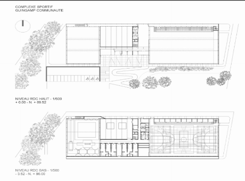
\includegraphics[width=.5\linewidth]{Ejemplo APA.png}
    \caption{\justifying \textit{Planta y zonificación guingamp. Adaptado de Stephane Chalmeau (2013). Guingamp agence d'architecture Robert et sur. Retrieved from http://www.archdaily.co/co/02-295165/guingamp-agence-d-architecture-robert-et-s}}
    \label{fig:Planta y zonificación guingamp}
\end{figure}

\subsubsection{Discusión (Opcional).}

Hace referencia a la evaluación e interpretación de las implicaciones de los resultados que arrojó el estudio. Se enfatiza en las consecuencias teóricas de los resultados y la validez de las conclusiones.

\chapter{Conclusiones}

Se presenta en forma exacta el aporte del desarrollo del trabajo en concordancia a la justificación presentada. Se describe en forma lógica, los resultados del trabajo, dando respuesta a los objetivos o propósitos planteados. Basado en los resultados recolectados, incluido el tratamiento estadístico o cualitativo. Se muestra en forma concisa los productos y/o resultados y se resaltan las contribuciones del trabajo al contexto local, regional, nacional e internacional, cuando aplique.

\chapter{Recomendaciones}

\begin{center}
    (Va en capitulo separado de las conclusiones y en este apartado se expresa las perspectivas del autor a fin de complementar con nuevas ideas a la investigación original)
\end{center}

\printbibliography

\appendix

\titleformat{\chapter}[display]
{\normalfont\centering\bfseries}
{\vspace{-17ex}}
{0pt}{}
[{\vspace{-5ex}}]

\chapter{Apéndice A: Tablas de datos}

\begin{center}
    (No lleva número de capitulo e inicia en hoja nueva)
\end{center}

Nota: Para los apéndices hay dos formas de presentarlos: si son menos de 27 se listan con las letras del alfabeto, además debe indicar cada título y la respectiva página. Si son más de 27 apéndices, se listan con números, además debe indicar cada título y no se coloca la página, remplazándolas así por el siguiente mensaje: “Ver apéndices adjuntos en el CD y pueden visualizarlos en base de datos de la Biblioteca UIS”, y por consiguiente, irían en una carpeta llamada “apéndices” adjunta en el CD.

\begin{figure}[H]
    \centering
    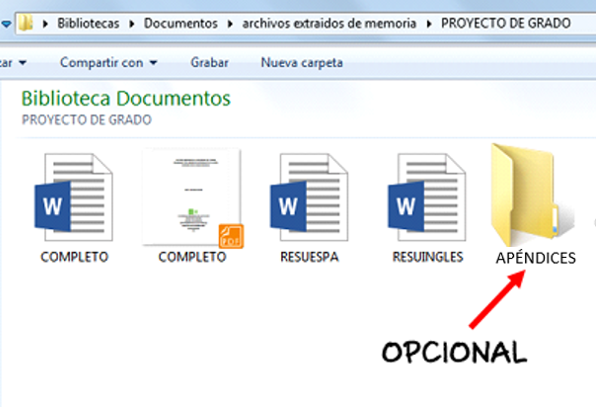
\includegraphics[width=.8\linewidth]{Recomendaciones Apendice.png}
    \label{fig:Recomendaciones Apéndice}
\end{figure}

Tener en cuenta que, en el uso de Normas APA no pueden ir contenidos en mayúscula (Incluyendo títulos), Sólo en mayúsculas las siglas y la cornisa.
Las recomendaciones y sugerencias para la elaboración de esta plantilla fueron obtenidas y adaptadas teniendo en cuenta el manual de publicaciones de la American Psychological Association 3ª. Edición [Traducida de la sexta en ingles]. Bogotá: Manual Moderno; 2010.



\end{document}